\section{How to use \toolname as a Slicing Tool}\label{sec:slice}

The \toolname slicing tool is available through the \pk{Tools
$\rightarrow$ Slicing Tool} menu option. The slicing tool
implements only a simple heuristic based on control-flow
information. As a future work, additional heuristics will be
implemented considering not only control-flow but also data-flow
information.

By changing to the slicing tool, the tester has to choose, among
the test cases, the ones that cause the fault and the ones that do
not reveal the fault. Based on the execution path of the failed
and succeed test cases, the tool highlights the part of the code
more probable to contain the fault.

%%%%%%%%%%%%%%%%%%%%%%%%%%%
\toolname uses a simple dynamic slice criterion, based on
control-flow information, to identify a subset of statements more
probable to contain the fault. The idea is (1) to compute the
failed set $F_S$ of \BG nodes (the execution path) of a failed
test case, which includes all statements executed by the failed
test case, (2) to compute the succeed set $S_S$ of \BG nodes
considering succeed test case(es), and (3) to calculate the
difference and the intersection of these sets to prioritize the
statements executed by the failed test case.

Using such an approach, instead of the complete set of \BG nodes
$N$ (which represents all statements of a method), the tester has
only to consider the subset of \BG nodes present in $F_S$, since
the other \BG nodes contains the statements not executed by the
failed test case and cannot contain the fault. Moreover,
considering the subset of nodes executed by the succeed test
cases, the most probably location of the fault is in the
statements executed by the failed test case but not executed by
the succeed test cases, \ie, the subset $F_S \setminus S_S$. Thus,
such a subset of statements has a highest priority and should be
analyzed first. If the fault is not located on this subset, due to
data dependence that can lead to a data-flow dependent fault, the
tester has to analyze the other statements executed by both the
failed and by the succeed test cases, \ie, the subset $F_S \cap
S_S$. In this way, we can provide an incremental search for the
fault, trying to reduce the time and the cost to locate the fault
in a program.

For example, consider the \BG presented in
Figure~\ref{fig-average-bcfg}. $N$ is the complete set of \BG
nodes ($N = \{0, 15, 34, 43, 54, 54.82, 60, 60.82, 74, 74.82, 79,
91, 97\}$). Suppose a failed test case that goes though \BG nodes
$F_S = \{0, 34, 15, 34, 43, 54, 54.82, 91, 97\}$ and a successful
test case that goes trough \BG nodes $S_S = \{0, 34, 43, 60,
60.82, 91, 97\}$. The most probably locations for the fault are in
the statements in nodes 15, 54 or 54.82, since they are only
executed by the failure test case ($F_S \setminus S_S$). If the
fault is not located on such statements, it will be found in the
other statements that compose the \BG nodes 0, 34, 43, 91 and 97
($F_S \cap S_S$). All the other \BG nodes have not to be analyzed.

The approach described above is based only on control-flow
information. The success of such an approach depends on which test
cases are selected as the successful test cases. It is important
to select successful test cases that execute the related
functionalities of the program as the ones executed by the failure
test case. In this way, the difference between the two sets $F_S$
and $S_S$ will result in subset with a few \BG nodes, reducing the
number of statements that have to be analyzed first.

In our Vending Machine example, test case \pk{0001} reveals the
fault and test case \pk{0006} does not. The tester can first
select only the failed test case, as illustrated in
Figure~\ref{fig:slice-test-case1}, and checks the execution path
of this test case as illustrated in
Figure~\ref{fig:slice-source-fail}. The red lines indicate the
statements that are executed by the failed test case and the white
lines indicates the statements not executed. Since there is a
fault, it must be located among these red statements.

\begin{figure}[!ht]
\begin{center}
\subfigure[]{\label{fig:slice-test-case1}\includegraphics[width=0.45\textwidth]{fig/slicing-fail-test-case.eps}}
\subfigure[]{\label{fig:slice-test-case6}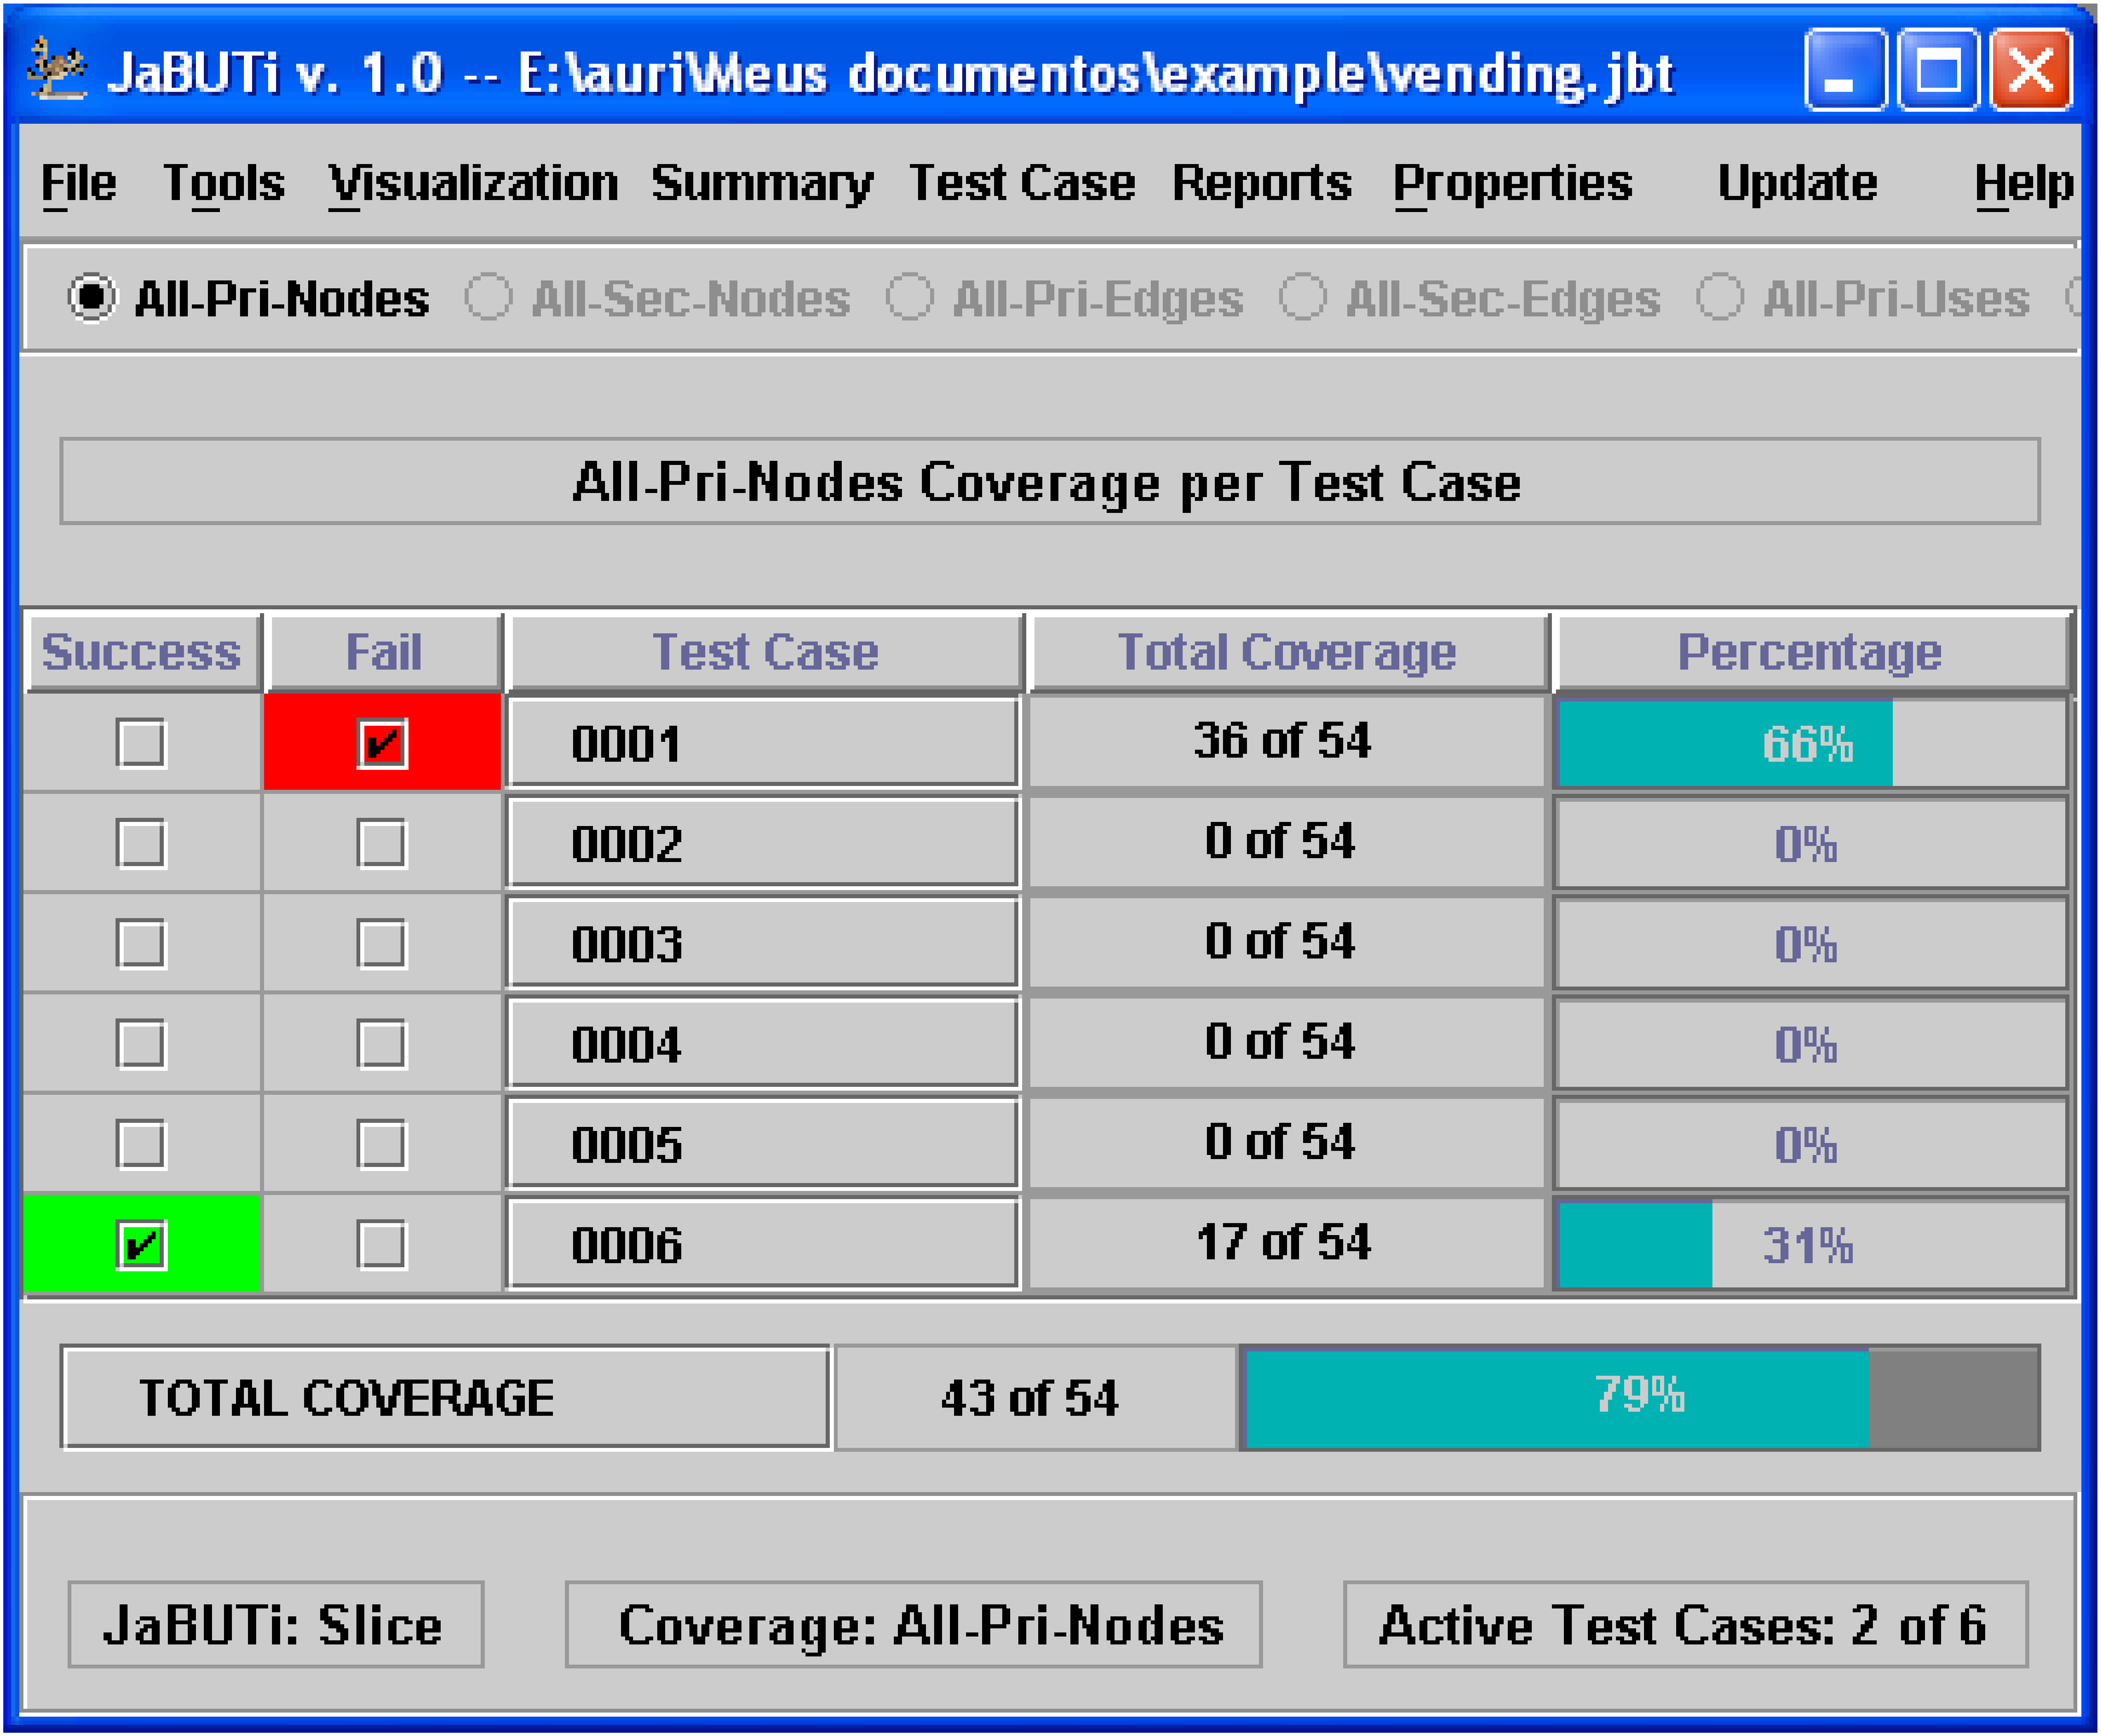
\includegraphics[width=0.45\textwidth]{fig/slicing-fail-1success-test-case.eps}}
\caption{Slicing tool test case selection: (a) only the failed
test case, and (b) a failed and a succeed test
cases.}\label{fig:slice-test-cases}
\end{center}
\end{figure}


After having observed the failed test case execution path, the
tester can enable one or more additional succeed test cases
(Figure~\ref{fig:slice-test-case6}), such that the tool can
identify, among the statements executed ny the failed test case,
the dice more probable to contain the fault (statements only
executed by the failed test case) and the ones less probable (the
ones executed for both the failed and the succeed test cases.)
Figure~\ref{fig:slice-source-fail-success} shows in yellow
(weight~1) the statements touched by test cases number \pk{0001}
and \pk{0006} and in red (weight~2) the statements only executed
by test case number~\pk{0001}.

The rationale of such an approach is that, in theory, the fault is
more probable to be located at the statements executed only by the
failed test case. Although, it can happen that the fault is
localized in other than the red statements, but the red points can
be used at least as a good starting point, trying to reduce the
search space for fault localization.

Once the fault is located and corrected, the testing activity is
restarted by creating a new project to revalidate the corrected
program. In this case, previous test sets can be used to
revalidate the behavior of the new program and also to check if
new faults were not introduced by the changes.

\begin{figure}[!ht]
\begin{center}
\subfigure[]{\label{fig:slice-source-fail}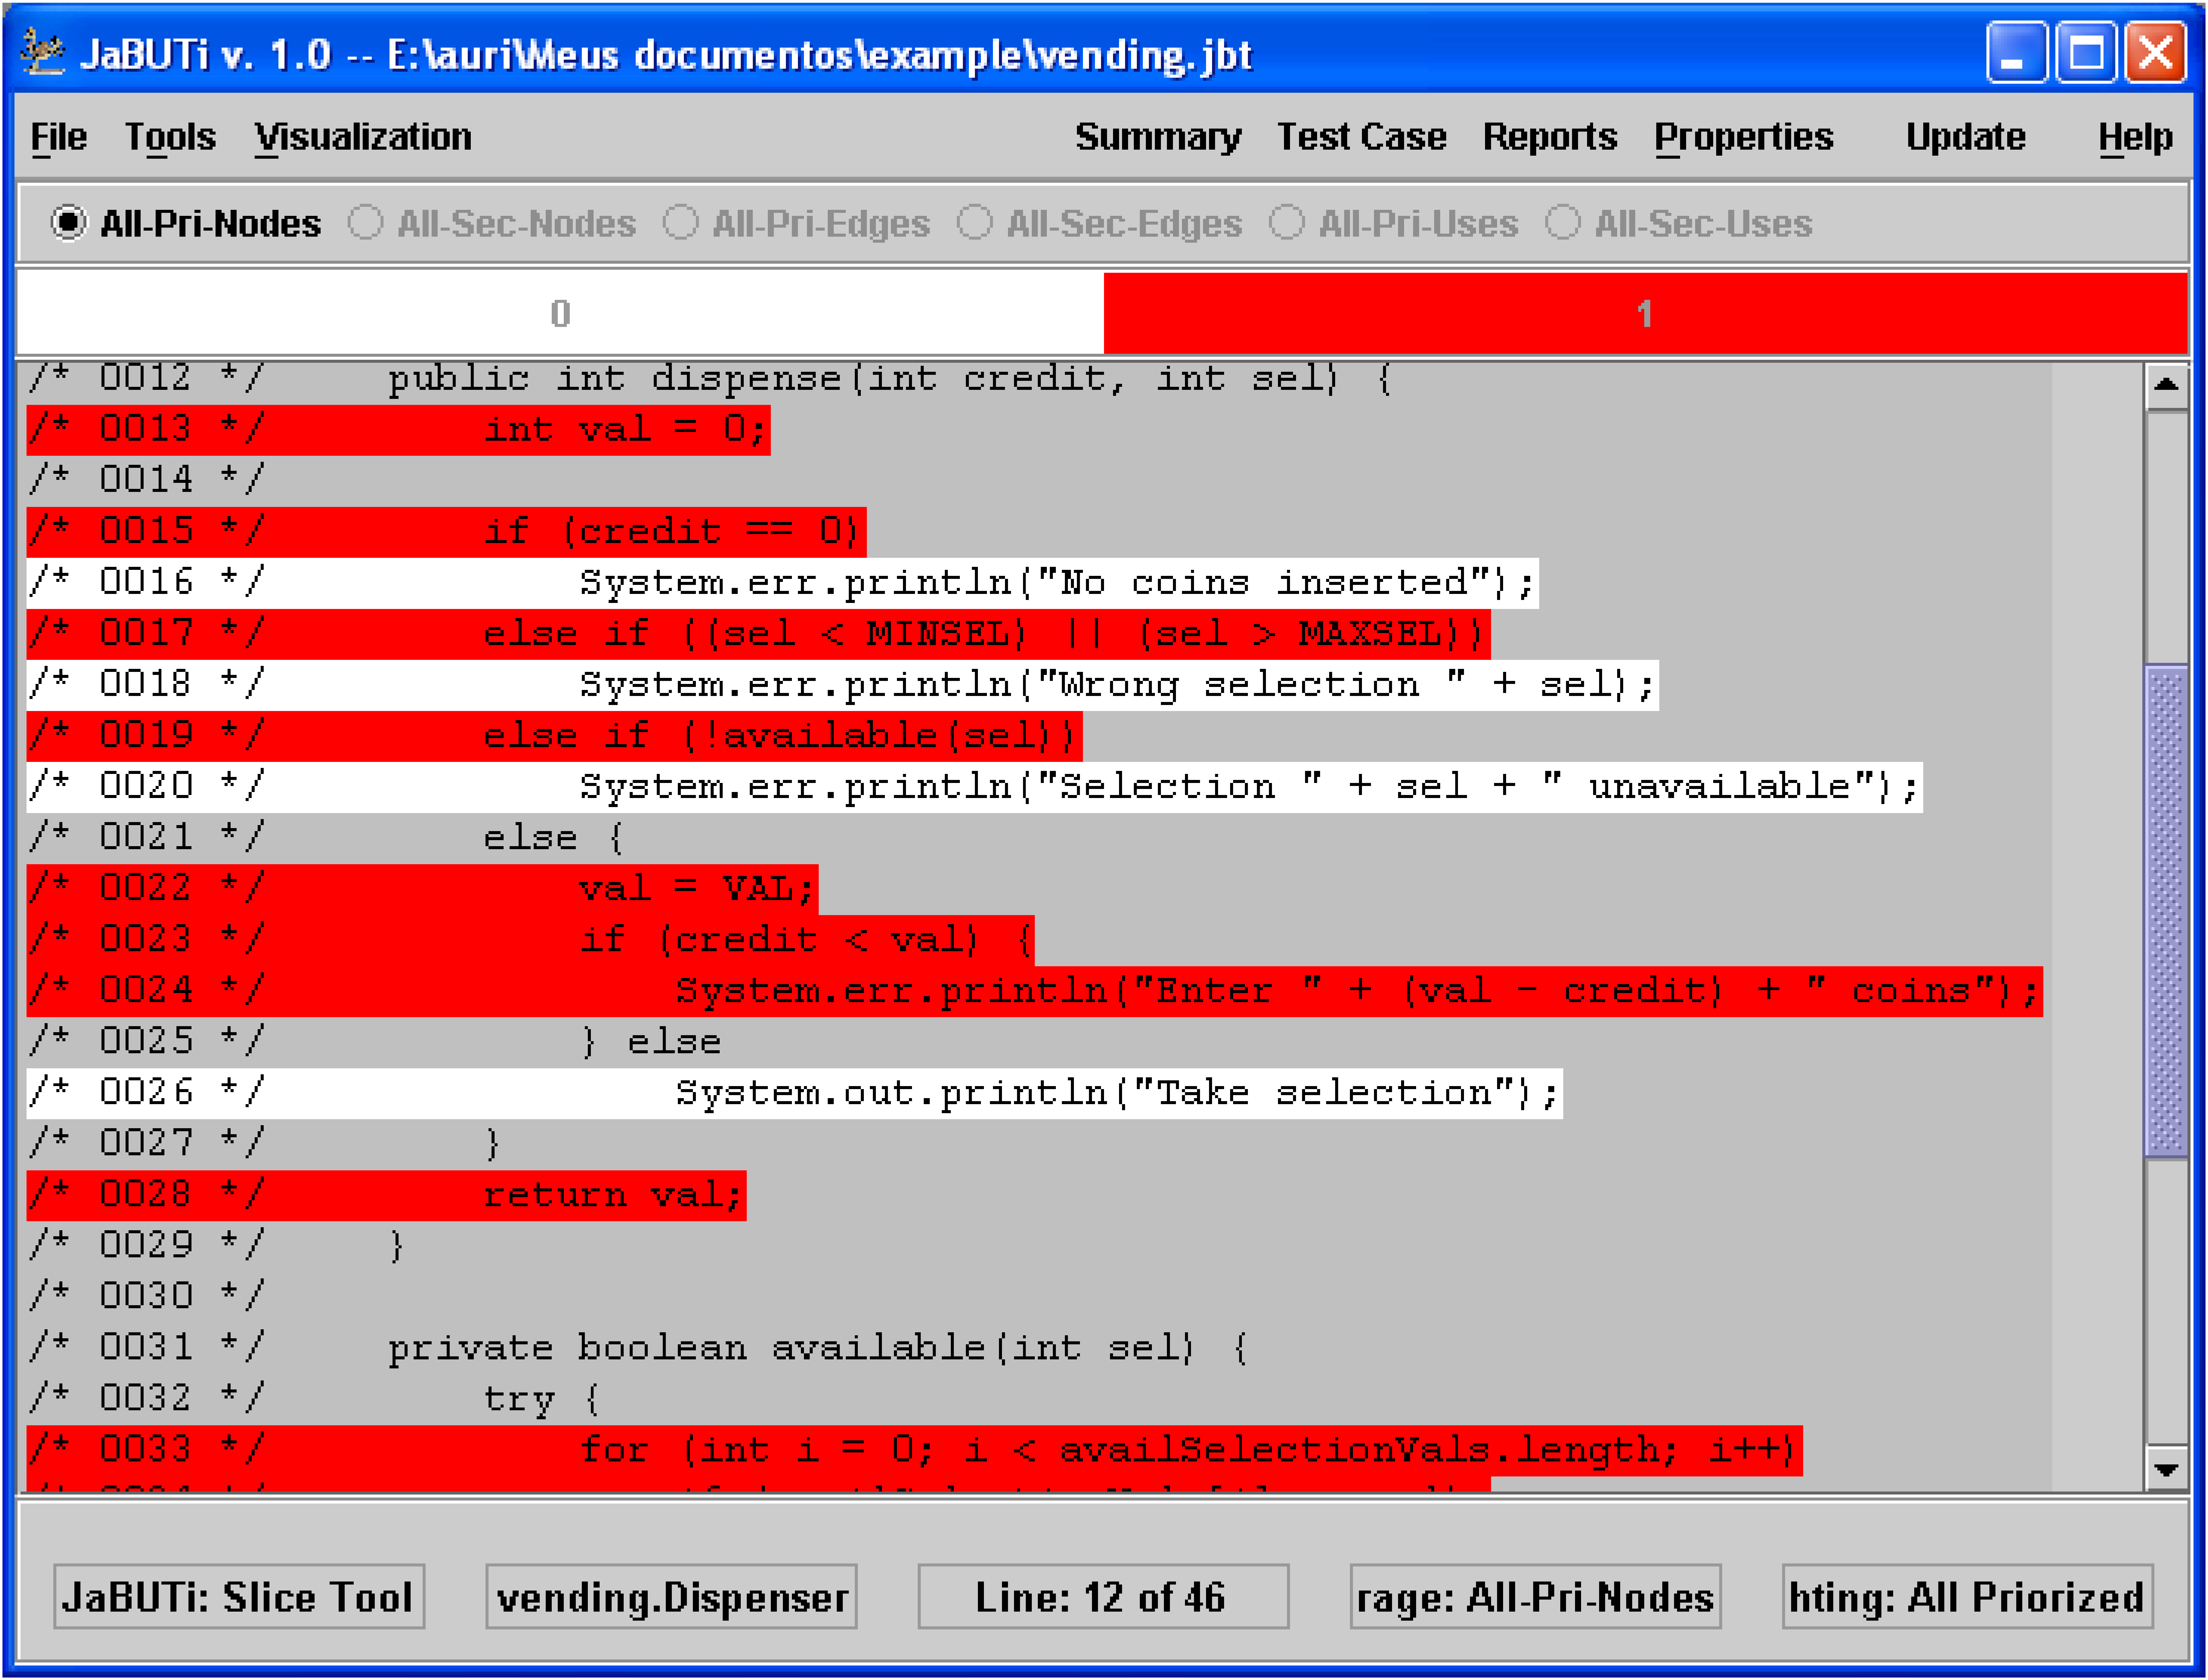
\includegraphics[width=0.45\textwidth]{fig/slicing-source-fail.eps}}
\subfigure[]{\label{fig:slice-source-fail-success}\includegraphics[width=0.45\textwidth]{fig/slicing-source-fail-1success.eps}}
\caption{Highlighted execution path: (a) fail test case execution
path, and (b) fail test case execution path intersected by the
success test case execution path.}\label{fig:slice-source}
\end{center}
\end{figure}

